
\section{An Embarrassingly Simple Baseline}
\label{sec:method_simple}

In the experiments of existing Transformer-based LTSF solutions ($T\gg1$), all the compared (non-Transformer) baselines are IMS forecasting techniques, which are known to suffer from significant error accumulation effects. We hypothesize that the performance improvements in these works are largely due to the DMS strategy used in them. 

\begin{figure}[h]
%\vspace{-0.2cm}
\begin{center}
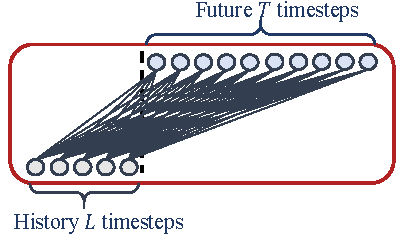
\includegraphics[width=0.32\textwidth]{img/linear.pdf}
\end{center}
\vspace{-0.3cm}
\caption{Illustration of the basic linear model.}
\vspace{-0.3cm}
\label{fig:Linear}
\end{figure}


To validate this hypothesis, we present the simplest DMS model via a temporal linear layer, named~\modelname, as a baseline for comparison. The basic formulation of \modelname directly regresses historical time series for future prediction via a weighted sum operation (as illustrated in Figure~\ref{fig:Linear}).
%
The mathematical expression is 
$\hat{X}_{i} = WX_i$, where $W\in \mathbb{R}^{T\times L}$ is a linear layer along the temporal axis. $\hat{X}_{i}$ and $X_i$ are the prediction and input for each $i_{th}$ variate. Note that \modelname shares weights across different variates and does not model any spatial correlations.




\modelname is a set of linear models. \textit{Vanilla Linear} is a one-layer linear model. To handle time series across different domains (e.g., finance, traffic, and energy domains), we further introduce two variants with two preprocessing methods, named \emph{DLinear} and \emph{NLinear}. 

\begin{itemize}

\item Specifically, \emph{DLinear} is a combination of a \emph{Decomposition} scheme used in Autoformer and FEDformer with linear layers. It first decomposes a raw data input into a trend component by a moving average kernel and a remainder (seasonal) component. Then, two one-layer linear layers are applied to each component, and we sum up the two features to get the final prediction.
%
By explicitly handling trend, \emph{DLinear} enhances the performance of a vanilla linear when there is a clear trend in the data. 
%
\item Meanwhile, to boost the performance of \modelname when there is a distribution shift in the dataset, \emph{NLinear} first subtracts the input by the last value of the sequence. Then, the input goes through a linear layer, and the subtracted part is added back before making the final prediction. The subtraction and addition in \emph{NLinear} are a simple normalization for the input sequence.
%
\end{itemize}
